\section{Application architecture}
\label{sec:application-architecture}

	\subsection{Prototypical application structure}
	
	This section presents the application architecture from the solution architecture point of view. A generic solution architecture is depicted in Figure \ref{fig:application-view}.
	
	The application architecture we present covers the application as a ``white box'': its internal component structure, services and interfaces with adjacent applications. Typically the solutions architecture takes the technology aspects into account, accounting for parts of the infrastructure.
	
    \begin{figure}[h]
		\centering
		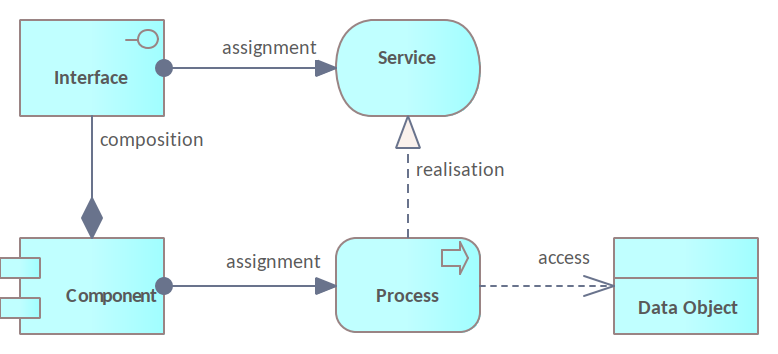
\includegraphics[width=.5\textwidth]{images/views/Application view.png}
		\caption{The prototypical application structure view}
		\label{fig:application-view}
	\end{figure}

	The central element of the application architecture is the \textit{application service}, which represents an application behaviour or functionality. The application services, from an inter-layer perspective, serve the processes in the business layer and provide support for their realisation. 
	
	
	The application services are realised through application processes. The processes have application components assigned to them signifying their place of encapsulation. Application components are modular and replaceable blocks encapsulating 
	implementation of application services and functionalities. In practice, for clarity, we take a shortcut, and say that the application services are realised through \textit{application components} directly.
	
	Components are said to expose interaction \textit{interfaces} which are modelled, in ArchiMate, as proper parts of the components. The interfaces are assigned to services signifying how the latter are to be accesses and consumed. 
	
	Also components, and processes they encapsulate, access \textit{data objects}, which are the passive components of the application architecture.

	The solution architecture presented in this section is an adaptation of the generic one. Here we focus on presenting for each business process, what application services are used to support it. Moreover, we are interested in grasping the difference in the application layer, between the current and new version of the business processes. 
	
	To do so we split the application view diagrams into three vertical lanes. The left lane hosts the current version of the business process and the application services and components that are used to support it. In the right lane, we place the new business process and the new application services and components that will have to be adopted for the digital transformation. The middle lane, hosts the services and components that are are currently employed and will be carried over into the new application architecture, they are common to the current and the new architectures.

	Next we present an overview of the application architecture, in terms of services alone, depicting how the asset lifecycle stages are served.
	
	\subsection{Current and new application service architecture}
	\label{sec:application-current}
	
	This section presents how the asset lifecycle stages are supported by the application services. The current application architecture is depicted in Figure \ref{fig:application-current} while the new one in Figure \ref{fig:application-new}. The services employed in each of the architectures are mostly the same, with a few exceptions. What differs more significantly is their utilisation in the asset lifecycle stages. For this reason we set them side by side to provide a contrasting image. 
	
	\begin{figure}
		\centering
		\begin{minipage}{0.485\textwidth}
			\centering
			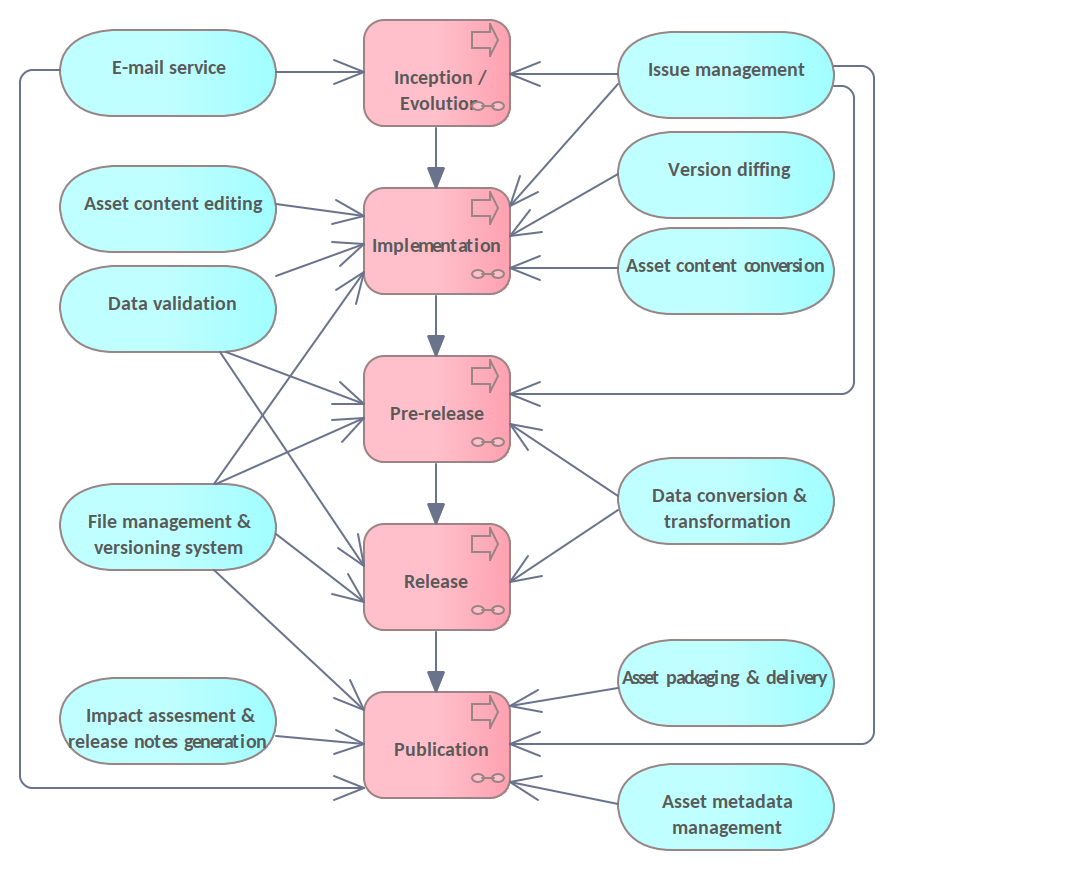
\includegraphics[width=1.3\textwidth]{images/application/Application Services (current).png}
			\caption{The application services that serve the current asset lifecycle}
			\label{fig:application-current}
		\end{minipage}\hfill
		\begin{minipage}{0.485\textwidth}
			\centering
			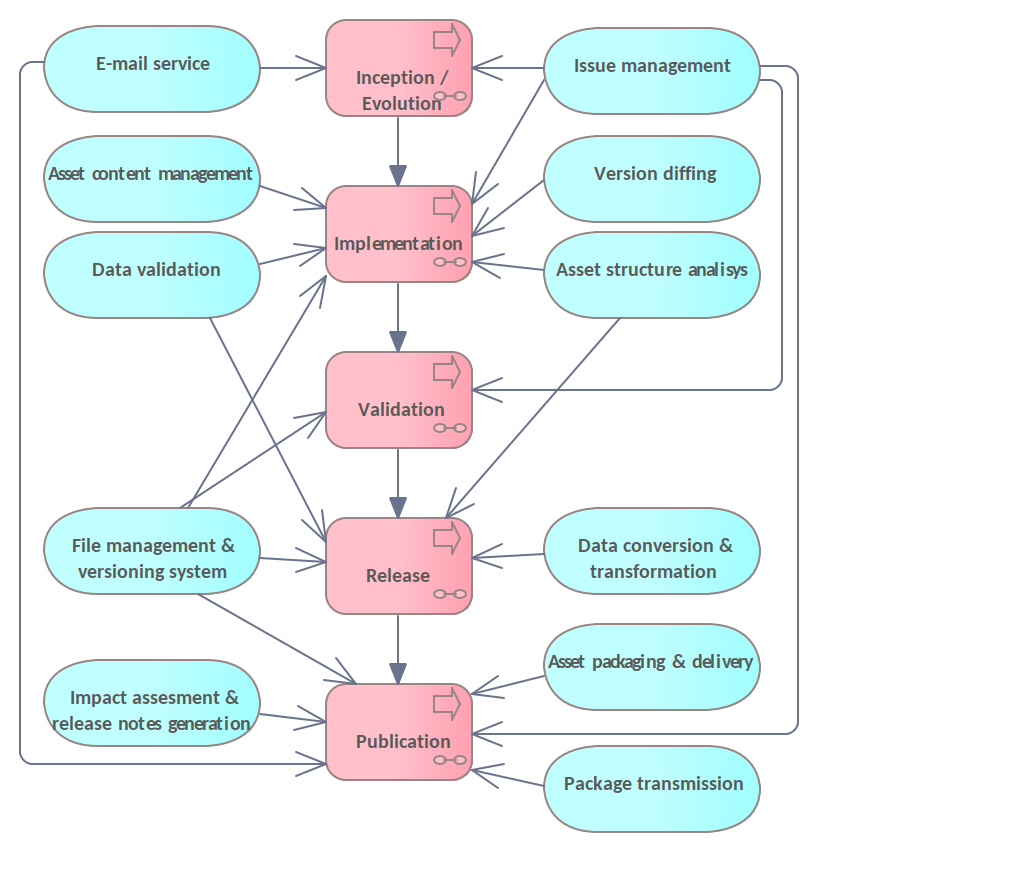
\includegraphics[width=1.3\textwidth]{images/application/Application Services (new).png}
			\caption{The application services that serve the new asset lifecycle}
			\label{fig:application-new}
		\end{minipage}
	\end{figure}
	
%	\begin{figure}[h]
%		\centering
%		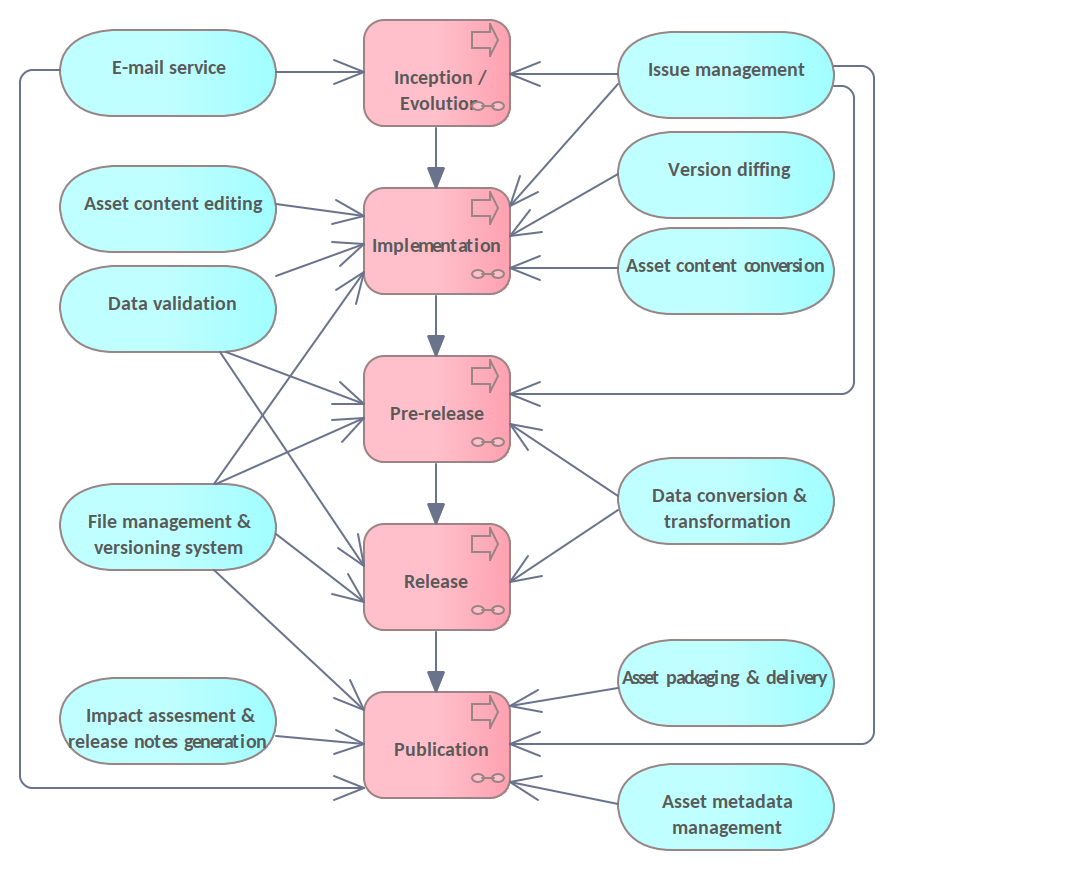
\includegraphics[width=.75\textwidth]{images/application/Application Services (current).png}
%		\caption{The application services that serve the current asset lifecycle}
%		\label{fig:application-current}
%	\end{figure}

	We start the description from the top of the diagram following the sequence of process stages. First is the \textit{e-mail service}. It represents the entire set of capabilities for sending emails covering both, the email server and the email client. This si realised via the Outlook system \citep{outlook}. 
	
	The \textit{issue management} service represents the capability of recording, documenting, and analysing a change request case in a distributed collaborative manner between multiple roles and actors. This is realised via the Jira system \citep{jira}. 
	
	\textit{Asset content editing} is the service which enables the documentalists in the team to modify asset content and hence implement the request cases. This service is realised by Excel desktop software \citep{excel}.
	
	The \textit{asset content conversion} service implements the conversion between Excel workbook and CAT-XML forms of the asset content. The two representations are equally expressive and the conversion process runs in both directions $ Excel \rightarrow XML $ and $XML \rightarrow Excel $.
	
	\textit{Version diffing} is a service which calculates and presents the difference between two versions of the same asset. The \textit{data validation} service, is self describing. It checks whether the asset content is correct. The asset content conversion, version diffing and data validation services are realised by components that compose the legacy workflow, which is currently in use.
	
	\textit{Asset document management} is provides capabilities for describing, storing and producing documents about assets in various human readable formats (e.g. HTML, PDF, docx). It also allows for document metadata management. Currently this capability is realised by PDF forms, called Asses Document Description (ADD), which are produced from XML-DITA sources \citep{dita-day2005introduction, dita-spec} using the Adobe FrameMaker \citep{framemaker} . 
	
	\textit{Asset metadata \& workflow management} is a service which centralises the flow of the automated processes. It is currently realised by the legacy workflow implementation. 
	
	The \textit{file management \& versioning} service enables storing the content and and tracing the evolution of assets. This service is realised by the SVN system \cite{svn}.
	
	The \textit{data transformation} service is self describing. It stands for a generic capability of transforming data from one form and format into another one. Currently this service is realised by a multitude of custom build transformation procedures, some of which are chained to produce the desired outcome. This service is realised by components that are part of the legacy system. 
	
	The \textit{asset packaging} service prepares the assets for transmission to the partner distribution systems, especially Cellar. It covers functionalities including assembling the necessary asset representations together with their documentation, generating the necessary technical metadata, and zipping the assets in a manner that is acceptable for the partner distribution systems. The type of package and the asset metadata description varies, yet among the most prominent ones are METS \citep{mets}, IMMC\footnote{see \url{https://op.europa.eu/en/web/eu-vocabularies/immc}} and DCAT \cite{dcat2}. 
	
	The last service to mention, that is employed in the current lifecycle process is the \textit{impact assessment \& release note generation} service. Its title is again self explanatory. The value it provides are the release notes, that are published with assets and describe the list of changes implemented in each version. The impact assessment is a type of report, which includes assessments for target stakeholders, which usually are service provides whose systems depend on the assets published by SU. These special impact assessments may target whether a given aspects of an asset have changed which may disrupt functioning systems. So a series of specific checkers and reports are produced to safeguard the partners. 
	
	The new application architecture (Figure \ref{fig:application-new}), as mentioned above, reconfigures how services are used across process stages. It replaces the asset content editing service by a new one which is \textit{asset content management}. This service is realised by a fully fledged semantic web editing system -- VocBench3 \citep{stellatovocbench}. In addition two more services are added: asset structure analysis and package transmission services.
	
	The \textit{asset structure analysis} implements an automatic fingerprinting of the asset structure which provides insight into how the managed asset is realised and instantiated. This fingerprinting serves as an indicator for the structural validation in the implementation step. For example, a missing or an extra property will be spotted with this service. 
	
	The \textit{package transmission} provides the possibility to automatically deliver and ingest the prepared packages into the dissemination system, rather than the publication officer performing this operation manually. 
	
%	\subsection{New application service architecture}
%	\label{sec:application-new}	

%	\begin{figure}[h]
%		\centering
%		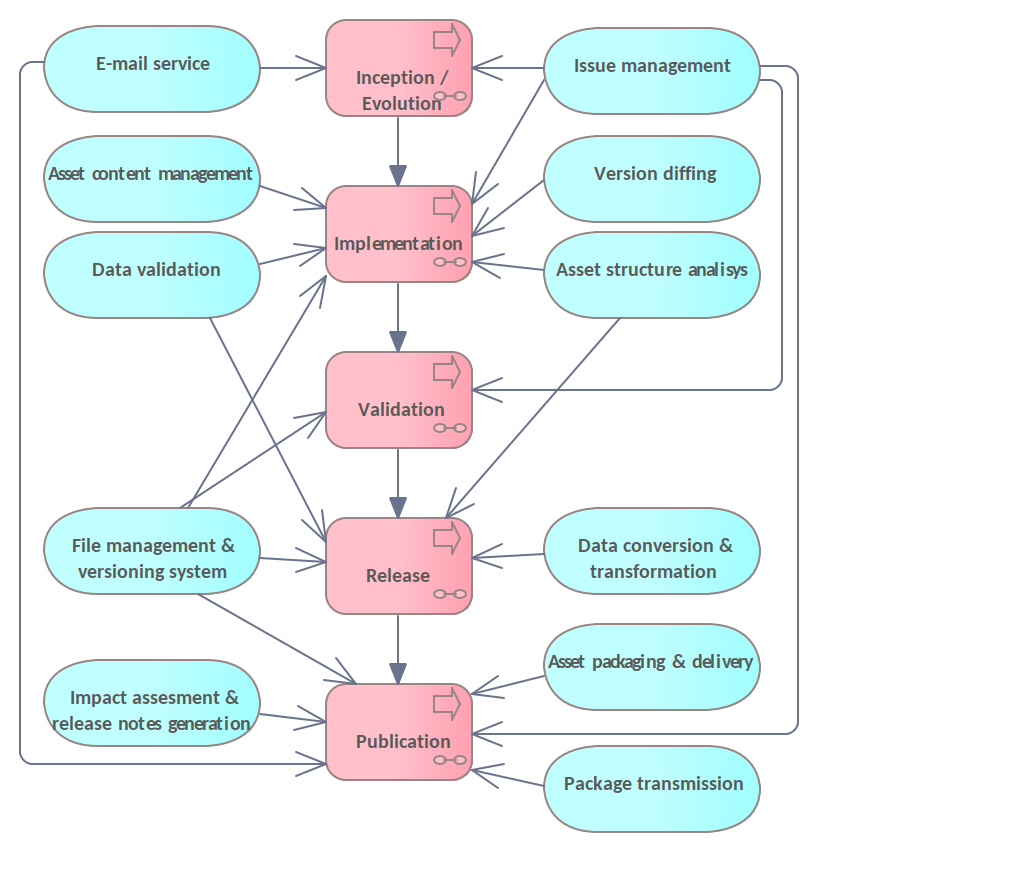
\includegraphics[width=.75\textwidth]{images/application/Application Services (new).png}
%		\caption{The application services that serve the new asset lifecycle}
%		\label{fig:application-new}
%	\end{figure}	
	
	\subsection{Inception and evolution services and components}
	\label{sec:evolution-application}	
	\begin{figure}[h]
		\centering
		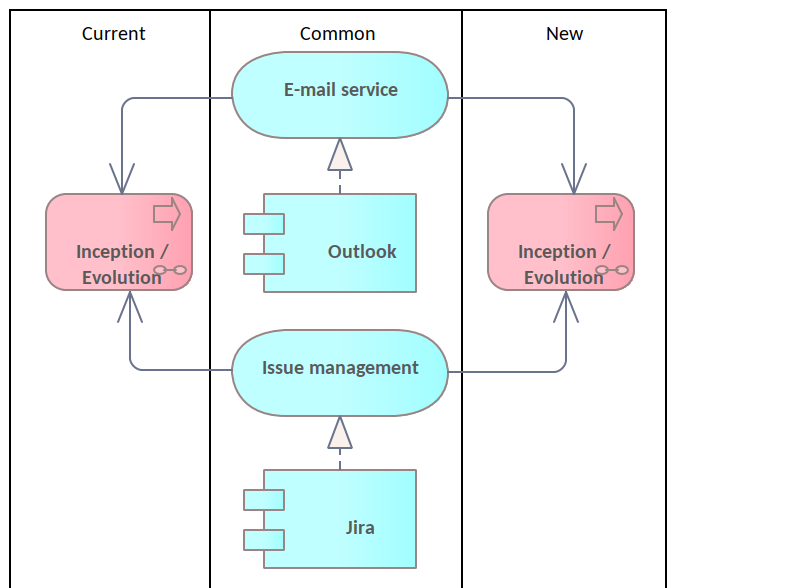
\includegraphics[width=.6\textwidth]{images/application/InceptionEvolution.png}
		\caption{The application services and components that serve the current and new inception and evolution stage}
		\label{fig:application-inception-evolution}
	\end{figure}

	\subsection{Implementation services and components}
	\label{sec:implementation-application}	
	\begin{figure}[h]
		\centering
		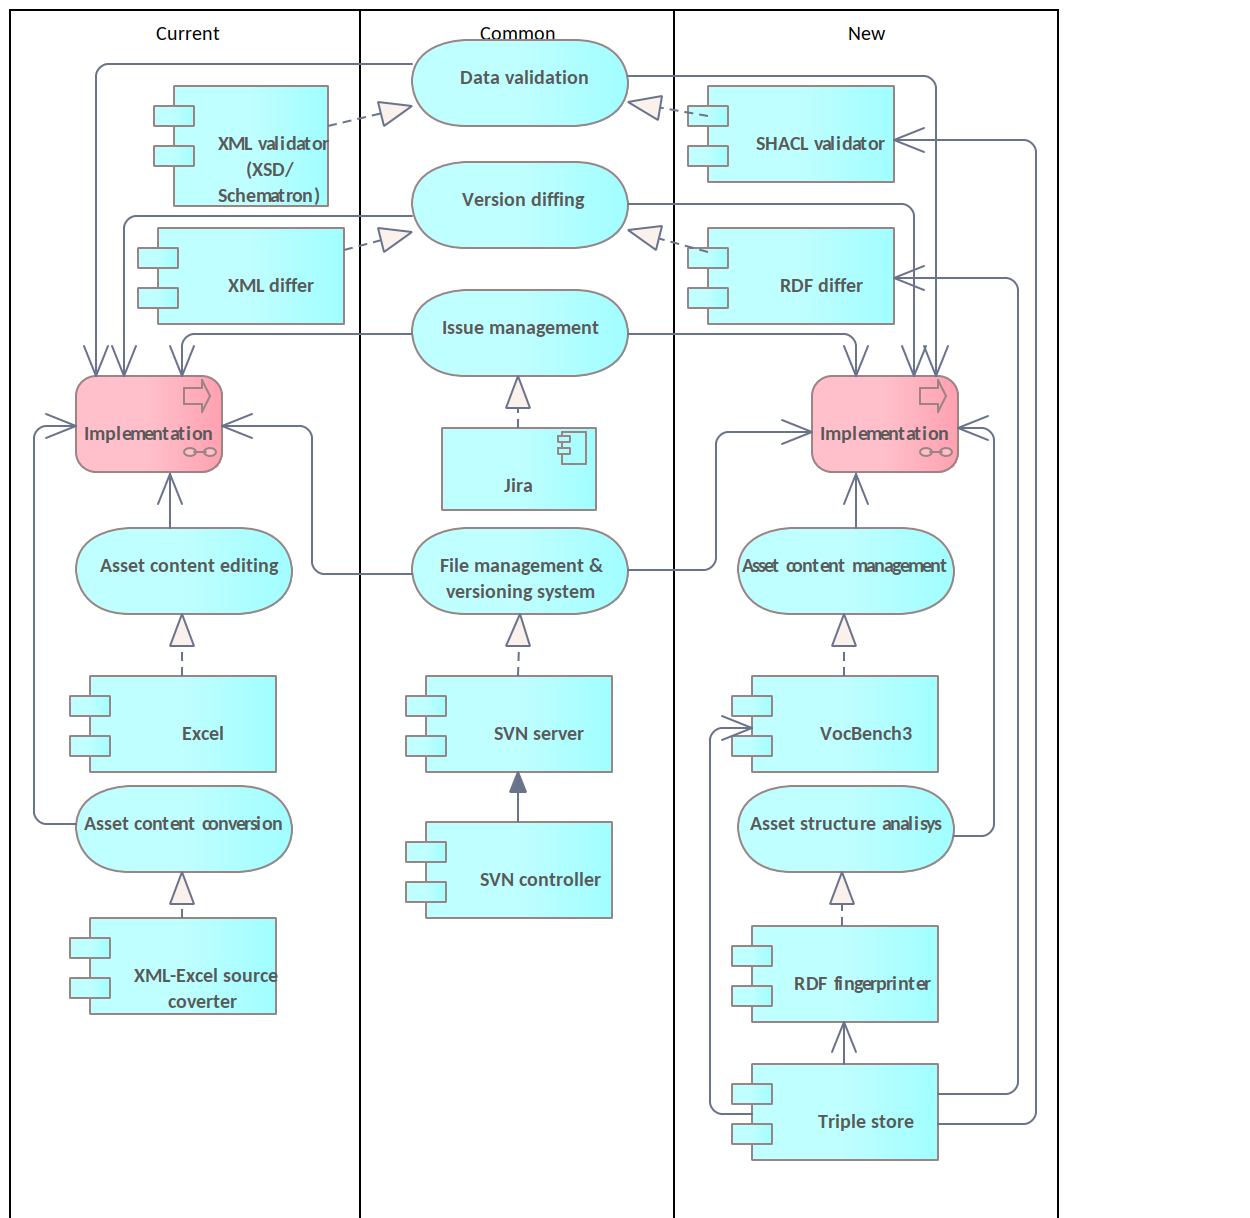
\includegraphics[width=.9\textwidth]{images/application/Implementation v3.png}
		\caption{The application services and components that serve the current and new implementation stage}
		\label{fig:application-implementation}
	\end{figure}
	
	\subsection{Pre-release and validation services and components}
	\label{sec:validation-application}
	\begin{figure}[h]
		\centering
		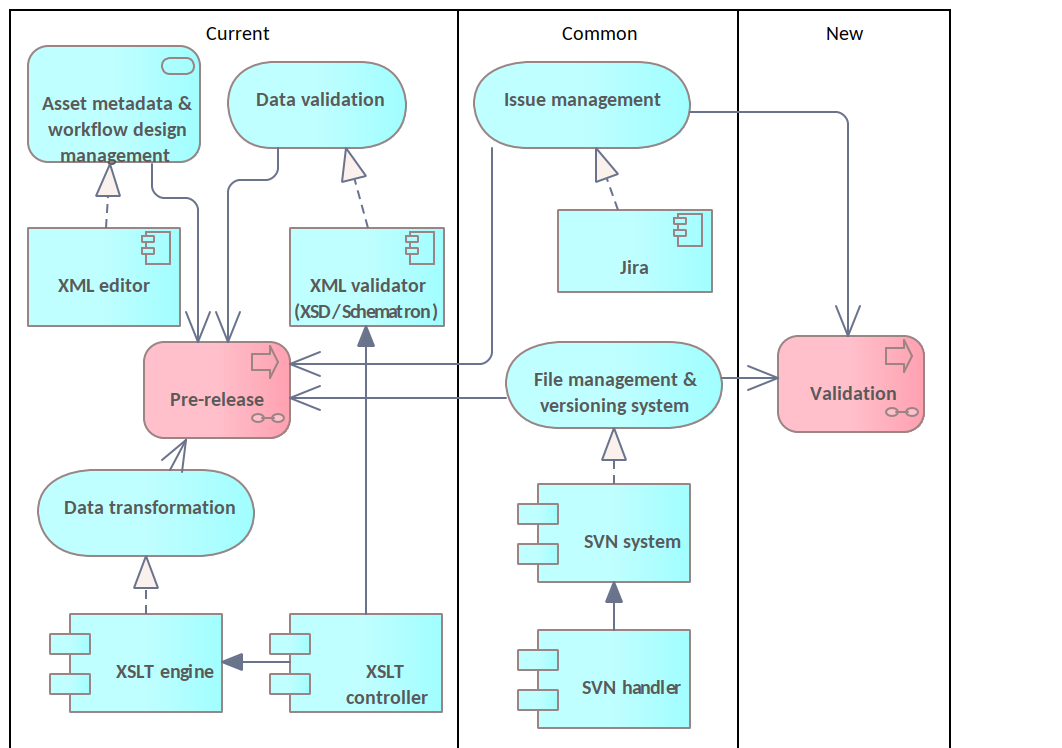
\includegraphics[width=.9\textwidth]{images/application/Validation & Pre-release v3.png}
		\caption{The application services and components that serve the current pre-release and the new validation stages}
		\label{fig:application-validation}
	\end{figure}

	\subsection{Release services and components}
	\label{sec:release-application}	
	
	\begin{figure}[h]
		\centering
		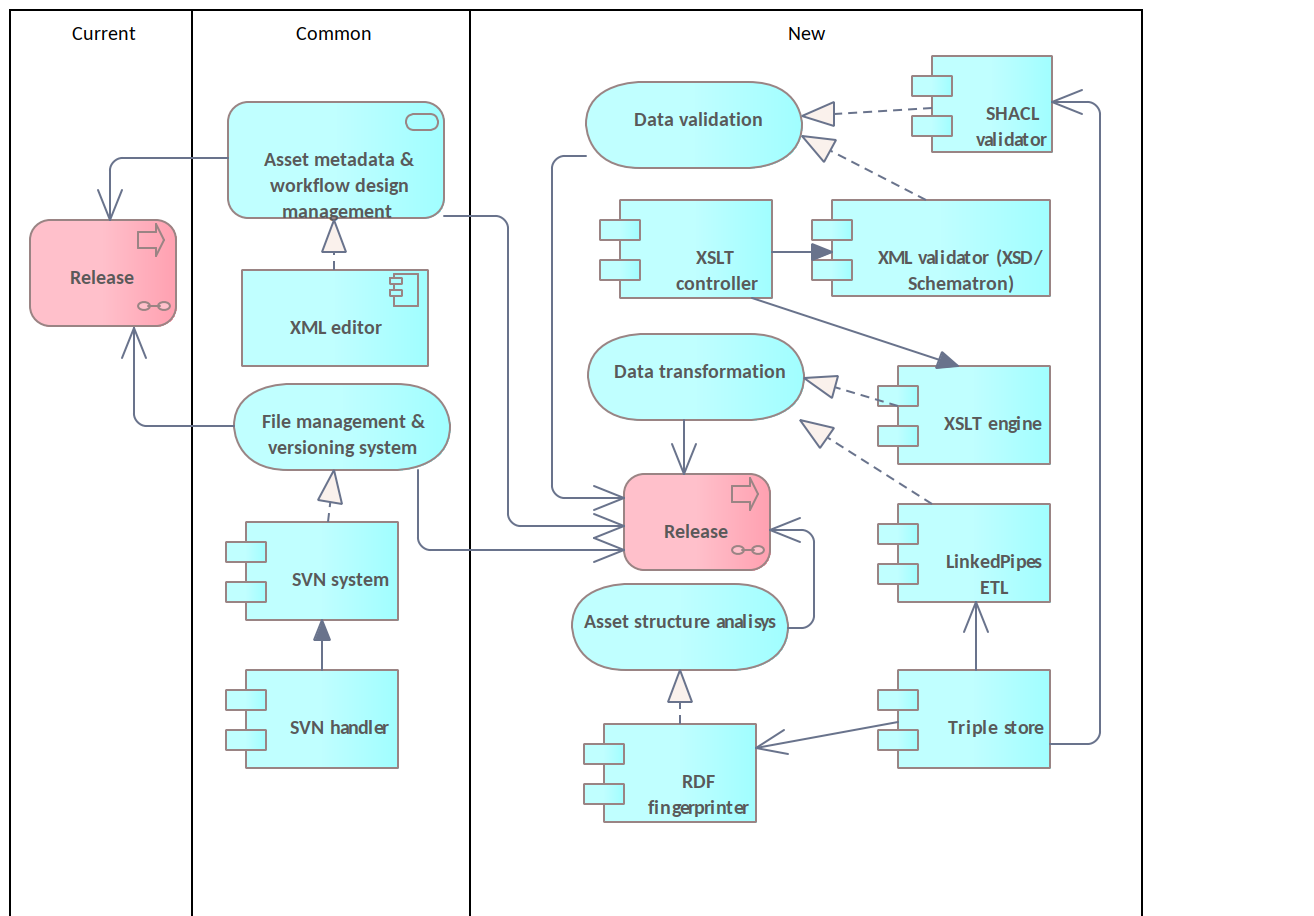
\includegraphics[width=.9\textwidth]{images/application/Release v3.png}
		\caption{The application services and components that serve the current and new release stage}
		\label{fig:application-release}
	\end{figure}
	
	\subsection{Publication services and components}
	\label{sec:publication-application}	
	
	\begin{figure}[h]
		\centering
		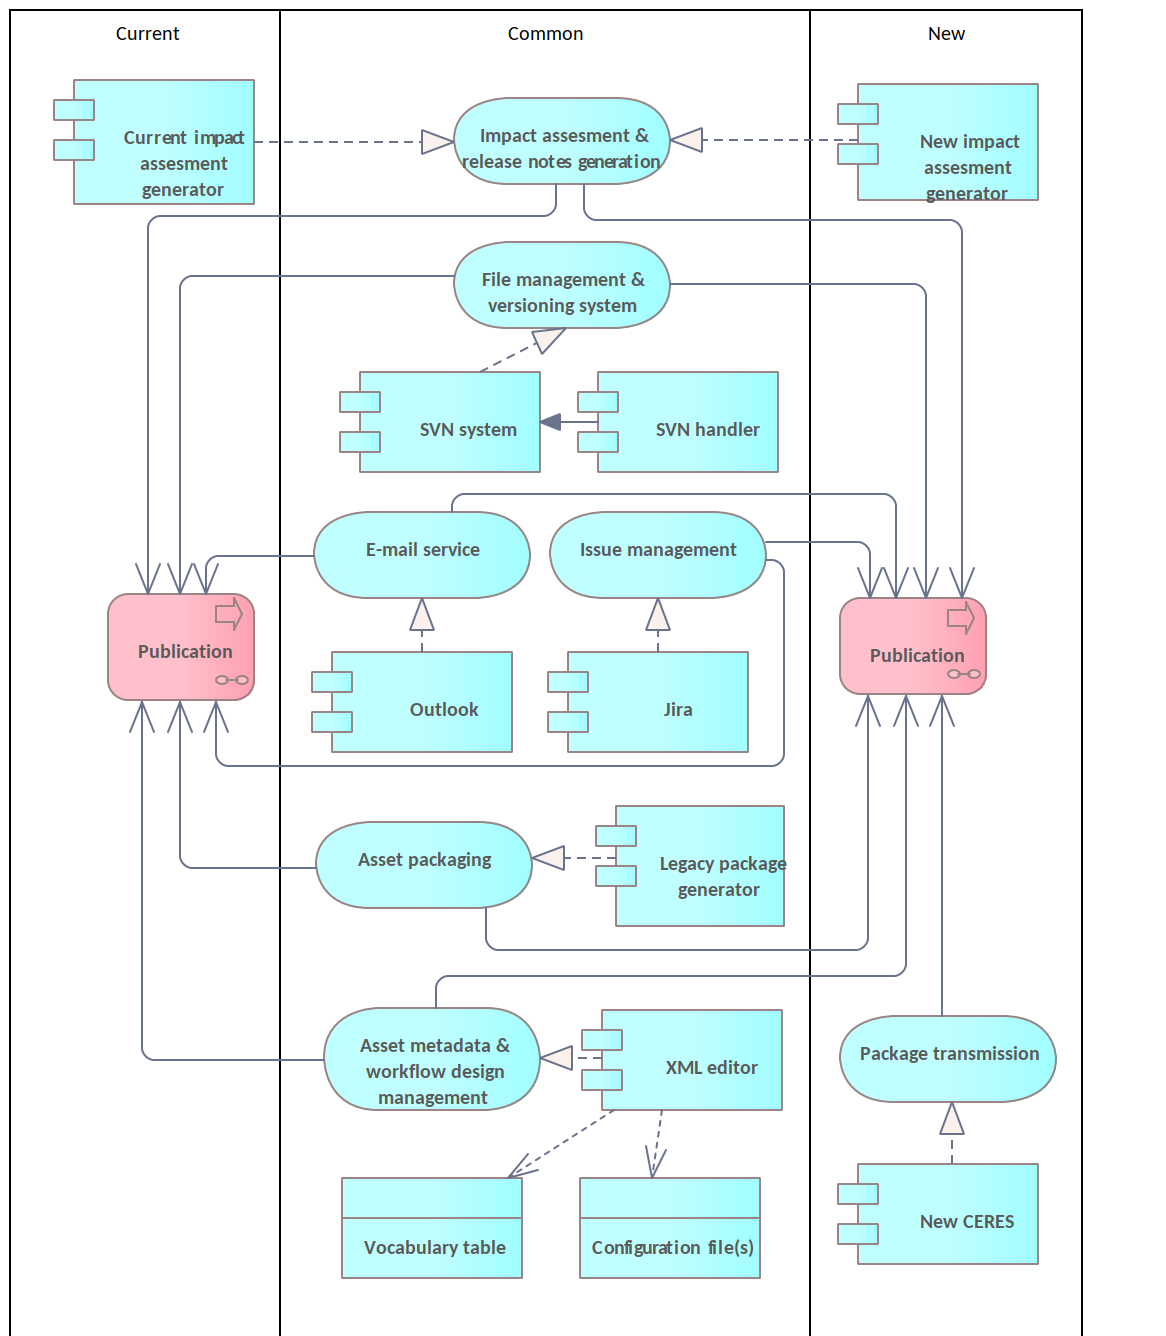
\includegraphics[width=.9\textwidth]{images/application/Publication v3.png}
		\caption{The application services and components that serve the current and new publication stage}
		\label{fig:application-publication}
	\end{figure}

	